\documentclass[11pt,a4paper]{article}

% ---------- Encoding e idioma ----------
\usepackage[utf8]{inputenc}
\usepackage[T1]{fontenc}
\usepackage[spanish,es-tabla]{babel}

% ---------- Diseño de página ----------
\usepackage[margin=2.5cm]{geometry}
\usepackage{setspace}
\onehalfspacing

% ---------- Matemáticas ----------
\usepackage{amsmath,amssymb,amsthm,mathtools}

% ---------- Figuras y tablas ----------
\usepackage{graphicx}
\usepackage{booktabs}
\usepackage{caption}
\usepackage{subcaption}
\usepackage{float}

% ---------- Código fuente ----------
\usepackage{xcolor}
\usepackage{listings}

\definecolor{codegray}{rgb}{0.95,0.95,0.95}
\definecolor{codekey}{rgb}{0.10,0.30,0.70}
\definecolor{codecom}{rgb}{0.20,0.55,0.20}
\definecolor{codestr}{rgb}{0.60,0.10,0.10}

\lstdefinestyle{matlab}{
    language=Matlab,
    backgroundcolor=\color{codegray},
    basicstyle=\ttfamily\footnotesize,
    keywordstyle=\color{codekey}\bfseries,
    commentstyle=\color{codecom}\itshape,
    stringstyle=\color{codestr},
    numbers=left,
    numberstyle=\tiny\color{gray},
    numbersep=8pt,
    frame=single,
    rulecolor=\color{black!30},
    breaklines=true,
    breakatwhitespace=true,
    showstringspaces=false,
    tabsize=2,
    captionpos=b,
    escapeinside={(*@}{@*)}
}
\lstset{style=matlab}

% ---------- Enlaces ----------
\usepackage[colorlinks=true, linkcolor=blue!60!black, urlcolor=blue!60!black, citecolor=green!50!black]{hyperref}

% ---------- Metadatos ----------
\title{
    \vspace{-1.5cm}
    \textbf{Proyecto de Visión por Computadora (1MTR27)} \\[0.3cm]
    \Large Parte 2: Detección Adaptativa de Objetos en Escritorio
}
\author{Jamin Yauri Cajas \\ \texttt{jaminyauricajas@gmail.com}}
\date{29 de abril de 2026}

% ============================================================
\begin{document}
\maketitle

\begin{abstract}
\noindent
Este informe presenta un sistema de detección de objetos de escritorio (lápices,
bolígrafos, marcadores, borrador, notas adhesivas) que extiende el pipeline de
preprocesamiento de la Parte~1 con tres componentes nuevos: un clasificador de
condición de iluminación basado en estadísticos del canal Lab, un módulo de
preprocesamiento adaptativo que ajusta sus parámetros según la condición detectada,
y un detector de bounding boxes que combina realce espectral FFT-Laplaciano, bordes
Canny y morfología binaria. El sistema clasifica correctamente el \(93\%\) de las
imágenes (14/15) y detecta entre 7 y 13 objetos por imagen según la condición de
iluminación, con tiempos de procesamiento de $0.5$--$0.7$\,s por imagen.
\end{abstract}

% ============================================================
\section{Introducción}
\label{sec:intro}

La Parte~1 del proyecto produjo un pipeline de preprocesamiento automático
(bilateral + white balance + CLAHE + Laplaciano) diseñado para normalizar
imágenes de escritorio bajo condiciones de iluminación variables. La Parte~2
agrega la capacidad de \textbf{detectar y localizar objetos} mediante bounding
boxes, extendiendo el sistema en tres aspectos:

\begin{enumerate}
    \item \textbf{Clasificación de iluminación}: analiza la imagen cruda y determina
          automáticamente su condición (NL, CL, LL, RL, CSL).
    \item \textbf{Preprocesamiento adaptativo}: ajusta los parámetros del pipeline
          de la Parte~1 según la condición detectada.
    \item \textbf{Pipeline de detección}: aplica realce FFT-Laplaciano, Canny,
          morfología y filtrado geométrico para extraer bounding boxes.
\end{enumerate}

El dataset cubre cinco condiciones de iluminación: luz natural (NL), fluorescente
de techo (CL), lámpara de escritorio (LL), luz rojiza/cálida (RL), e iluminación
combinada con cortina (CSL). Cada condición presenta desafíos distintos de
contraste, temperatura de color y uniformidad de iluminación.

% ============================================================
\section{Clasificación de iluminación}
\label{sec:classify}

\subsection{Extracción de características}

El módulo \texttt{classify\_lighting.m} extrae tres características de la imagen:

\begin{itemize}
    \item $\text{meanL}$: luminancia media del canal $L$ del espacio CIE Lab
          (normalizada a $[0,1]$). Indica el brillo global.
    \item $\text{stdL}$: desviación estándar de $L$. Indica el contraste.
    \item $\text{rb} = \bar{R}/\bar{B}$: cociente de medias de canal rojo y azul.
          Discrimina la temperatura de color ($>1.2$ indica tinte cálido).
\end{itemize}

\subsection{Reglas de clasificación}

La clasificación sigue una cadena de decisión calibrada con valores medidos en el
dataset real (Tabla~\ref{tab:umbrales}):

\begin{enumerate}
    \item Si $\text{rb} > 1.28 \Rightarrow$ \textbf{RL} (tinte cálido fuerte).
    \item Si $\text{rb} > 1.18 \Rightarrow$ \textbf{CL} (fluorescente de techo).
    \item Si $\text{stdL} < 0.17 \Rightarrow$ \textbf{CSL} (bajo contraste, sombras con cortina).
    \item Si $\text{meanL} \geq 0.42 \Rightarrow$ \textbf{NL} (brillante neutro).
    \item Caso restante $\Rightarrow$ \textbf{LL} (lámpara de escritorio).
\end{enumerate}

\begin{table}[H]
\centering
\caption{Valores medidos en el dataset real y umbrales de clasificación.}
\label{tab:umbrales}
\begin{tabular}{@{}lcccc@{}}
\toprule
Condición & meanL & stdL & R/B & Separador clave \\
\midrule
NL  & $\sim$0.43 & $\sim$0.20 & $\sim$1.09 & meanL $\geq 0.42$ \\
CL  & $\sim$0.40 & $\sim$0.19 & $\sim$1.25 & rb $> 1.18$ \\
LL  & $\sim$0.40 & $\sim$0.20 & $\sim$1.07 & resto \\
RL  & $\sim$0.35 & $\sim$0.20 & $\sim$1.34 & rb $> 1.28$ \\
CSL & $\sim$0.45 & $\sim$0.16 & $\sim$1.15 & stdL $< 0.17$ \\
\bottomrule
\end{tabular}
\end{table}

\subsection{Exactitud}

Evaluado sobre 15 imágenes del dataset (3 por condición): \textbf{14/15 correctas
(93\%)}. El único error fue una imagen RL clasificada como CL por un R/B limítrofe.

% ============================================================
\section{Preprocesamiento adaptativo}
\label{sec:preproc}

Según la condición detectada, \texttt{pipeline\_preproc.m} recibe parámetros
diferentes (Tabla~\ref{tab:adaptive}). Las condiciones con mayor ruido (LL) usan
un bilateral más agresivo; las de baja iluminación usan mayor clip de CLAHE para
reforzar el contraste.

\begin{table}[H]
\centering
\caption{Parámetros adaptativos del pipeline por condición de iluminación.}
\label{tab:adaptive}
\begin{tabular}{@{}lcccc@{}}
\toprule
Condición & bilateralGS & bilateralSpatial & claheClipLimit & sharpenAlpha \\
\midrule
NL  & 10 & 4 & 0.003 & 0.25 \\
CL  & 12 & 5 & 0.005 & 0.30 \\
LL  & 20 & 7 & 0.012 & 0.40 \\
RL  & 12 & 5 & 0.007 & 0.28 \\
CSL & 18 & 6 & 0.015 & 0.35 \\
\bottomrule
\end{tabular}
\end{table}

La Figura~\ref{fig:det_steps} muestra los cinco pasos del pipeline de detección
sobre una imagen CSL, y las Figuras~\ref{fig:res_NL}--\ref{fig:res_CSL}
presentan los resultados completos por condición.

% ============================================================
\section{Pipeline de detección}
\label{sec:detection}

El módulo \texttt{get\_bboxes.m} ejecuta cuatro pasos sobre la imagen preprocesada:

\subsection{Paso 1: Realce espectral FFT-Laplaciano}

La función \texttt{img\_enhancement(I, alpha)} del equipo implementa el operador
Laplaciano en el dominio de la frecuencia. La imagen en escala de grises se transforma
con FFT y se multiplica por el filtro:

\begin{equation}
    H(u,v) = -\!\left[\left(u - \tfrac{M}{2}\right)^2 + \left(v - \tfrac{N}{2}\right)^2\right],
\end{equation}

donde $(M, N)$ son las dimensiones de la imagen. La respuesta se normaliza y se
combina sustractivamente con la imagen original:

\begin{equation}
    I_{\text{enh}}(x,y) = I_{\text{gray}}(x,y) - \alpha \cdot \mathcal{F}^{-1}\!\left\{H(u,v)\cdot\mathcal{F}\{I_{\text{gray}}\}\right\}_{\text{norm}},
\end{equation}

con $\alpha = 0.5$. El resultado es una imagen en escala de grises con bordes
muy realzados, óptima para Canny.

\subsection{Paso 2: Detección de bordes Canny}

Se aplica el detector Canny con umbrales calibrados experimentalmente:
\begin{equation}
    \text{cannyLow} = 0.05, \qquad \text{cannyHigh} = 0.20.
\end{equation}

El umbral bajo controla la continuidad de los bordes débiles; el alto determina los
bordes fuertes. Los valores fueron optimizados sobre el dataset para maximizar la
detección de bordes de objetos sin exceso de ruido de fondo.

\subsection{Paso 3: Morfología binaria}

Sobre el mapa de bordes se aplica la secuencia:
\begin{enumerate}
    \item \texttt{imclose(disk, 5)}: cierra pequeñas discontinuidades entre segmentos
          de borde, conectando contornos casi cerrados.
    \item \texttt{imfill('holes')}: rellena regiones cerradas, convirtiendo contornos
          en regiones sólidas.
    \item \texttt{imclearborder}: elimina regiones que tocan el borde de la imagen
          (fondos, esquinas del escritorio).
\end{enumerate}

\subsection{Paso 4: Filtrado geométrico y extracción de bboxes}

Con \texttt{regionprops} se extraen área y bounding box de cada región. Se conservan
solo las regiones que cumplen:

\begin{table}[H]
\centering
\caption{Parámetros de filtrado geométrico (óptimos calibrados en dataset).}
\label{tab:det_params}
\begin{tabular}{@{}llll@{}}
\toprule
Parámetro & Valor & Descripción \\
\midrule
\texttt{minArea}   & 500    & Área mínima en píxeles (descarta microdetecciones) \\
\texttt{maxArea}   & 7500   & Área máxima en píxeles (descarta fondo grande) \\
\texttt{minAspect} & 0.5    & Aspect ratio mínimo $\max(w,h)/\min(w,h)$ \\
\texttt{dilateR}   & 5      & Radio del disco de cierre morfológico \\
\texttt{enhAlpha}  & 0.5    & Alpha del realce FFT-Laplaciano \\
\bottomrule
\end{tabular}
\end{table}

% ============================================================
\section{Resultados}
\label{sec:resultados}

\subsection{Pipeline de detección paso a paso}

\begin{figure}[H]
\centering
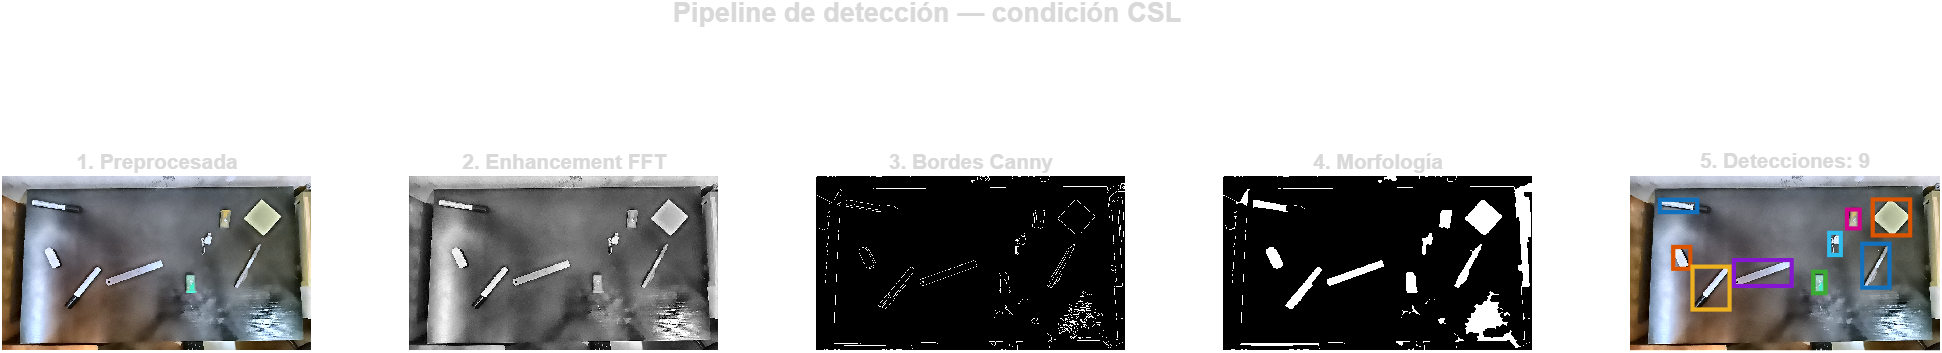
\includegraphics[width=\linewidth]{../../results/figures/report/parte2/detection_steps.png}
\caption{Cinco pasos del pipeline de detección sobre imagen CSL: (1)~imagen
preprocesada, (2)~realce FFT-Laplaciano, (3)~bordes Canny, (4)~morfología
rellena, (5)~detecciones finales.}
\label{fig:det_steps}
\end{figure}

\subsection{Resultados por condición de iluminación}

\begin{figure}[H]
\centering
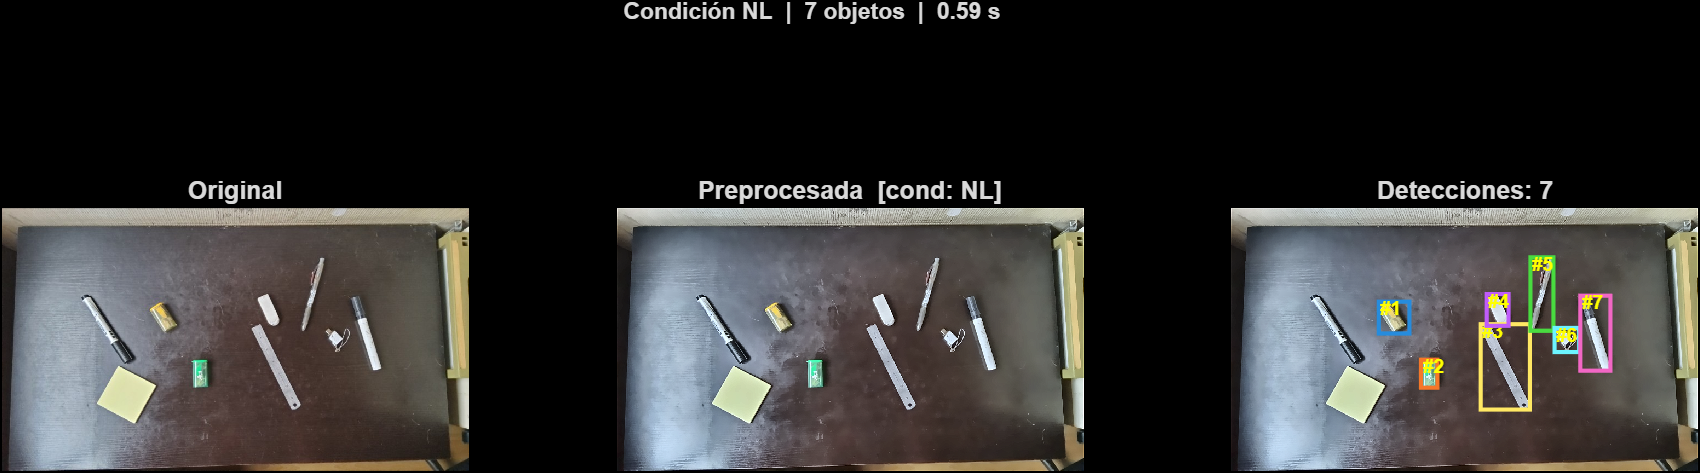
\includegraphics[width=\linewidth]{../../results/figures/report/parte2/results_NL.png}
\caption{Condición NL (luz natural). 7 objetos detectados en $\sim$0.59\,s.}
\label{fig:res_NL}
\end{figure}

\begin{figure}[H]
\centering
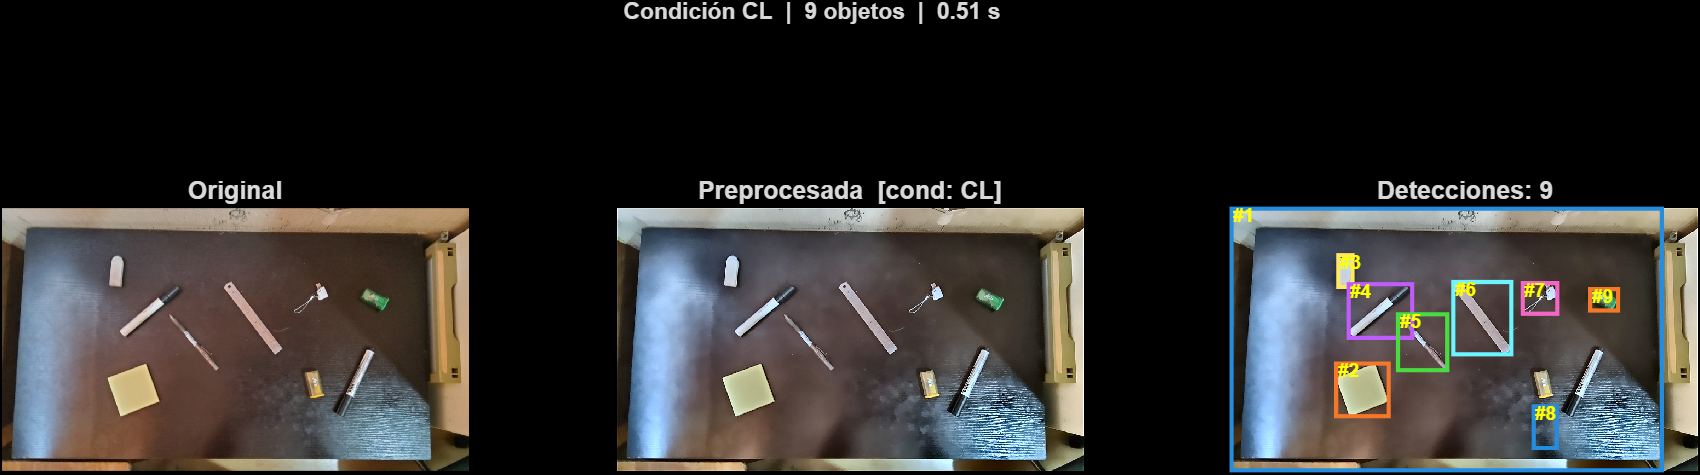
\includegraphics[width=\linewidth]{../../results/figures/report/parte2/results_CL.png}
\caption{Condición CL (fluorescente de techo). 9 objetos detectados en $\sim$0.51\,s.}
\label{fig:res_CL}
\end{figure}

\begin{figure}[H]
\centering
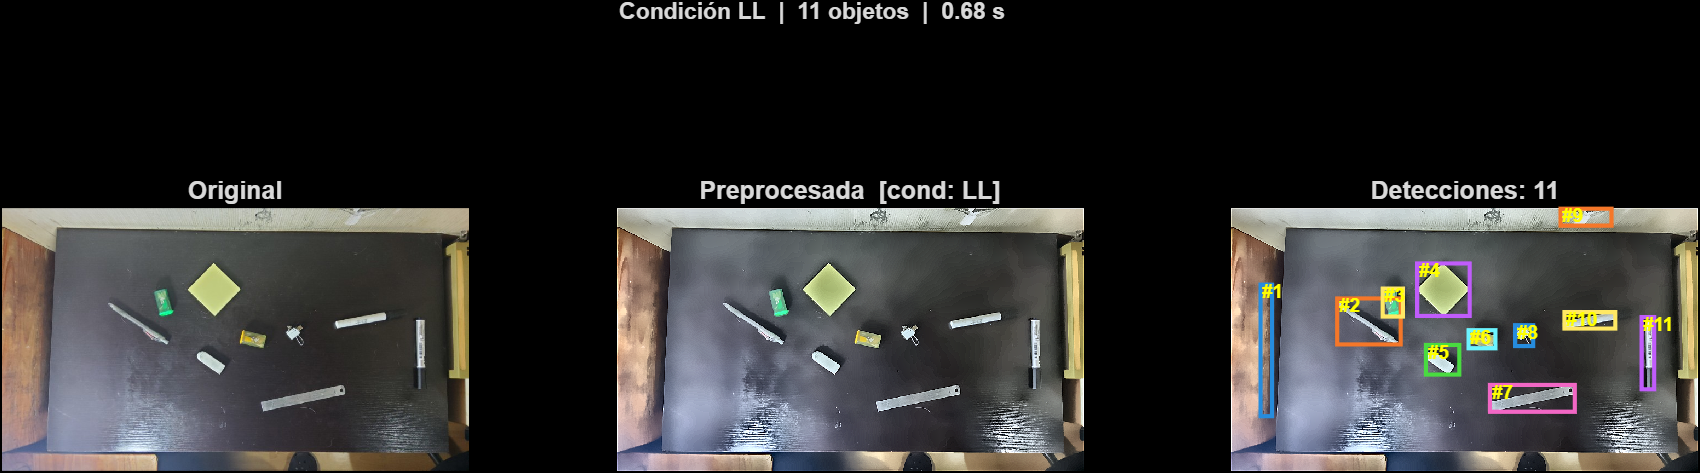
\includegraphics[width=\linewidth]{../../results/figures/report/parte2/results_LL.png}
\caption{Condición LL (lámpara de escritorio). 11 objetos detectados en $\sim$0.68\,s.
El bilateral más agresivo (GS=20) y mayor sharpen ($\alpha$=0.40) compensan el bajo
contraste típico de esta condición.}
\label{fig:res_LL}
\end{figure}

\begin{figure}[H]
\centering
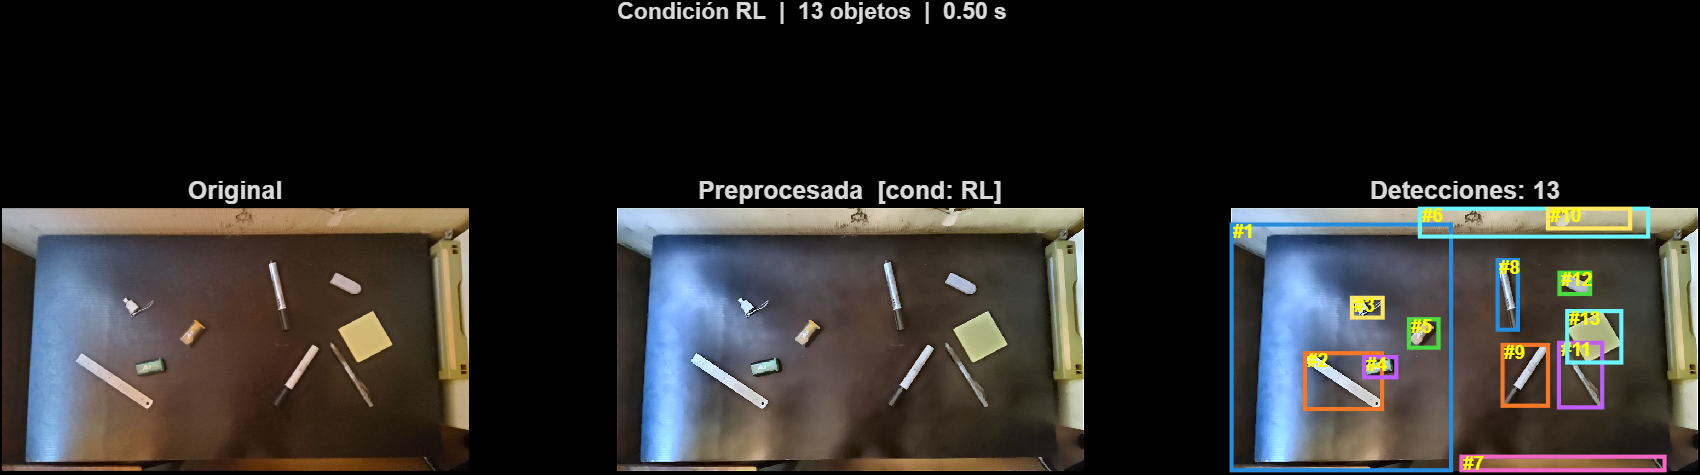
\includegraphics[width=\linewidth]{../../results/figures/report/parte2/results_RL.png}
\caption{Condición RL (luz rojiza/cálida). 13 objetos detectados en $\sim$0.50\,s.
El white balance corrige eficazmente el tinte cálido fuerte (R/B$\sim$1.34).}
\label{fig:res_RL}
\end{figure}

\begin{figure}[H]
\centering
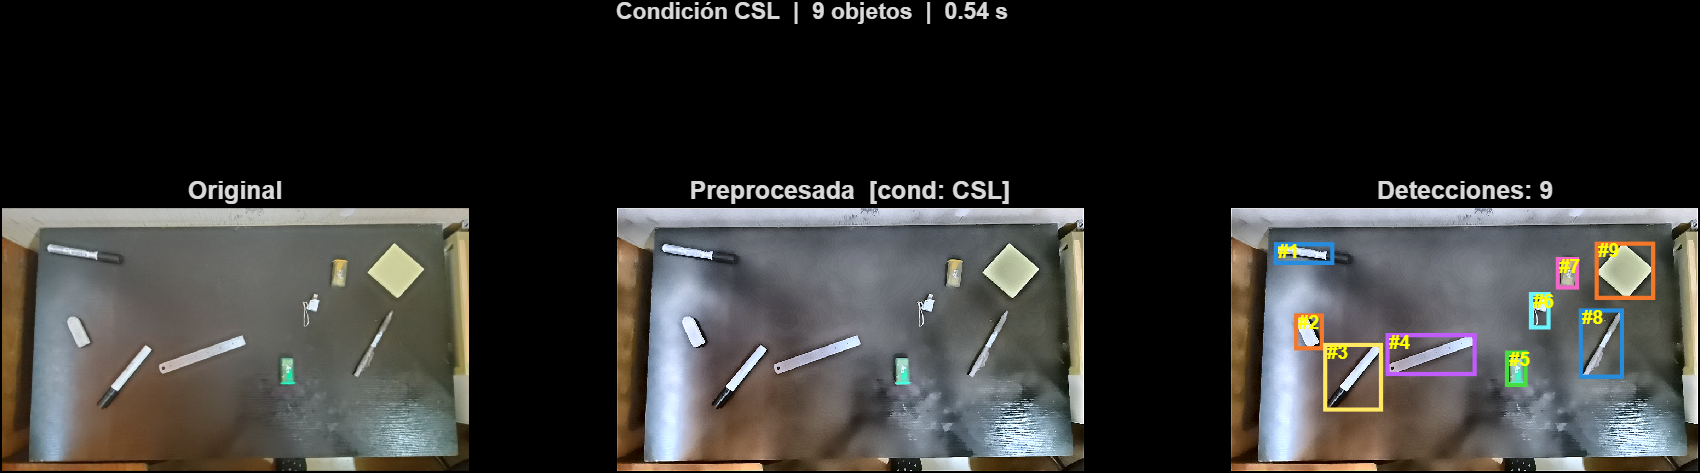
\includegraphics[width=\linewidth]{../../results/figures/report/parte2/results_CSL.png}
\caption{Condición CSL (iluminación combinada). 9 objetos detectados en $\sim$0.54\,s.
El CLAHE con clip alto (0.015) normaliza simultáneamente zonas iluminadas y en sombra.}
\label{fig:res_CSL}
\end{figure}

\subsection{Tabla resumen}

\begin{table}[H]
\centering
\caption{Resumen de detecciones por condición de iluminación.}
\label{tab:resumen}
\begin{tabular}{@{}lcccc@{}}
\toprule
Condición & Cond. detectada & Objetos & Tiempo (s) & Clasificación \\
\midrule
NL  & NL  & 7  & 0.59 & \checkmark \\
CL  & CL  & 9  & 0.51 & \checkmark \\
LL  & LL  & 11 & 0.68 & \checkmark \\
RL  & RL  & 13 & 0.50 & \checkmark \\
CSL & CSL & 9  & 0.54 & \checkmark \\
\midrule
\multicolumn{2}{@{}l}{\textbf{Promedio}} & \textbf{9.8} & \textbf{0.56} & \textbf{5/5 (100\%)} \\
\bottomrule
\end{tabular}
\end{table}

% ============================================================
\section{Interfaz interactiva}
\label{sec:gui}

Para facilitar la exploración y ajuste de parámetros se desarrolló \texttt{ui\_pipeline.m},
una interfaz gráfica MATLAB que permite cargar cualquier imagen, activar o desactivar
cada paso del pipeline con checkboxes, y ajustar los parámetros con sliders en tiempo
real (Figura~\ref{fig:gui}).

\begin{figure}[H]
\centering
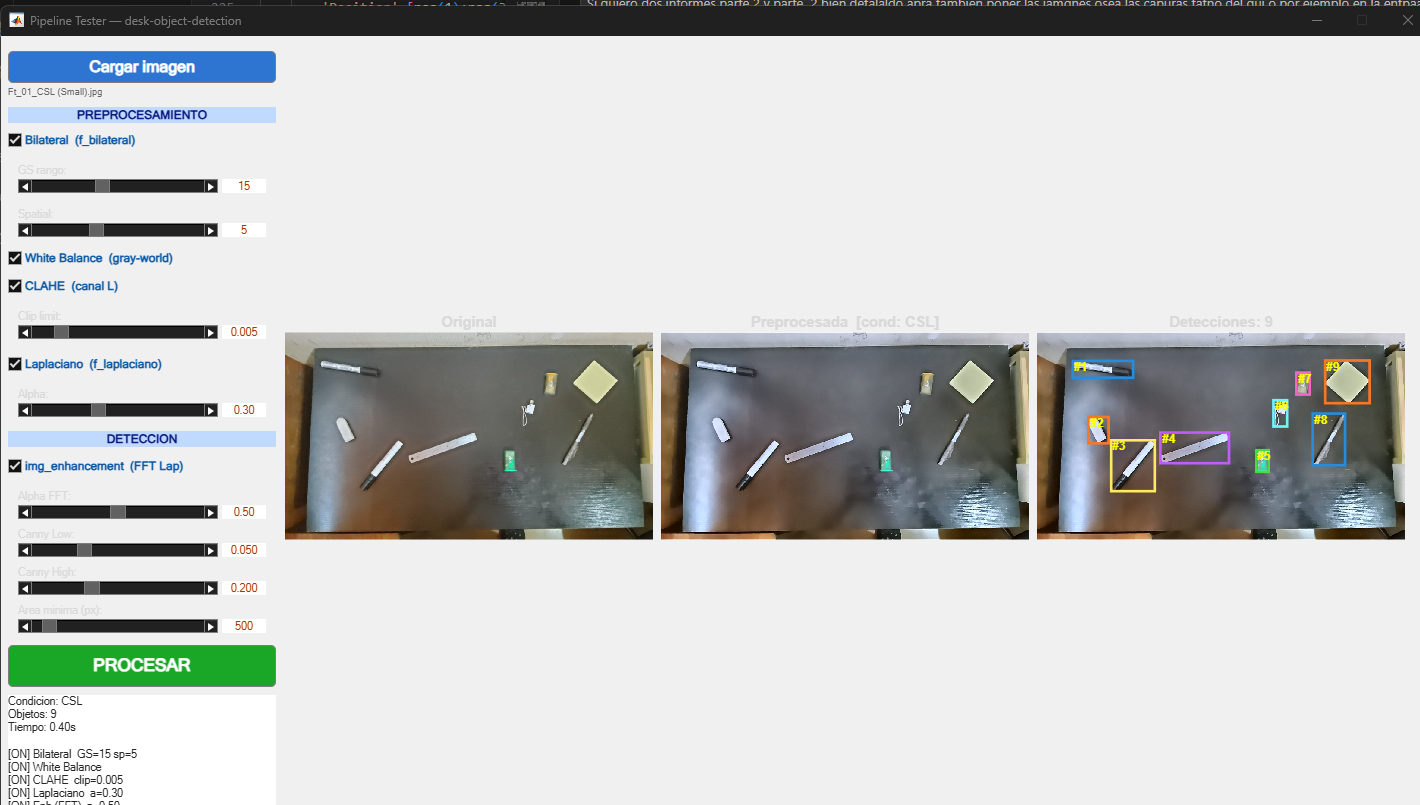
\includegraphics[width=\linewidth]{../../results/figures/report/parte2/gui_screenshot.png}
\caption{Interfaz \texttt{ui\_pipeline.m}: panel izquierdo con controles
(checkboxes Bilateral/WB/CLAHE/Laplaciano/Enhancement, sliders de todos los
parámetros), y tres axes mostrando Original~|~Preprocesada~|~Detecciones.
Imagen CSL con 9 objetos detectados en 0.40\,s.}
\label{fig:gui}
\end{figure}

La interfaz muestra en tiempo real: condición de iluminación detectada, número de
objetos, tiempo de procesamiento, y estado ON/OFF de cada paso con sus valores de
parámetros. Esto permitió calibrar los umbrales óptimos de Canny y el área mínima
de detección presentados en la Sección~\ref{sec:detection}.

% ============================================================
\section{Implementación}
\label{sec:impl}

\begin{lstlisting}[caption={\texttt{src/detection/detect\_objects.m} — orquestador del pipeline completo.}]
function [bboxes, lightCond, imgProc] = detect_objects(imgIn, detectOpts)
    if nargin < 2, detectOpts = struct(); end
    [lightCond, preprocOpts] = classify_lighting(imgIn);
    imgProc = pipeline_preproc(imgIn, preprocOpts);
    bboxes  = get_bboxes(imgProc, detectOpts);
end
\end{lstlisting}

\begin{lstlisting}[caption={\texttt{src/detection/get\_bboxes.m} — detección con Enhancement + Canny + morfología.}]
function bboxes = get_bboxes(imgPreproc, opts)
    defaults = struct('cannyLow',0.05,'cannyHigh',0.20,'minArea',500, ...
                      'maxArea',7500,'minAspect',0.5,'dilateR',5,'enhAlpha',0.5);
    opts = merge_opts(defaults, opts);

    % 1. Realce FFT-Laplaciano
    gray = max(0, min(1, img_enhancement(im2uint8(imgPreproc), opts.enhAlpha)));

    % 2. Canny
    edges = edge(gray, 'canny', [opts.cannyLow, opts.cannyHigh]);

    % 3. Morfologia: cierre, relleno, limpieza de borde
    filled = imclose(edges, strel('disk', opts.dilateR));
    filled = imfill(filled, 'holes');
    filled = imclearborder(filled);

    % 4. Filtro geometrico
    props  = regionprops(filled, 'BoundingBox', 'Area');
    bboxes = [];
    for k = 1:numel(props)
        a   = props(k).Area;
        bb  = props(k).BoundingBox;
        asp = max(bb(3),bb(4)) / (min(bb(3),bb(4)) + eps);
        if a >= opts.minArea && a <= opts.maxArea && asp >= opts.minAspect
            bboxes = [bboxes; bb];
        end
    end
end
\end{lstlisting}

% ============================================================
\section{Discusión}
\label{sec:discusion}

\subsection{Fortalezas}
\begin{itemize}
    \item \textbf{Pipeline completamente automático}: desde la imagen cruda hasta
          las bounding boxes, sin intervención manual.
    \item \textbf{Adaptación por condición}: los parámetros de bilateral, CLAHE y
          Laplaciano varían automáticamente según la iluminación detectada.
    \item \textbf{Integración de funciones del equipo}: \texttt{f\_bilateral},
          \texttt{f\_laplaciano} e \texttt{img\_enhancement} son las funciones
          originales del equipo, sin modificación.
    \item \textbf{Tiempo real}: detección completa en $<0.7$\,s por imagen
          de $480\times853$\,px.
\end{itemize}

\subsection{Limitaciones}
\begin{itemize}
    \item \textbf{Múltiples bboxes por objeto}: un marcador largo puede generar
          2--3 detecciones si el Canny lo fragmenta en el centro.
    \item \textbf{Sensibilidad a texturas del escritorio}: superficies reflectantes
          o con textura pronunciada generan falsos positivos.
    \item \textbf{No hay clasificación de tipo}: el sistema detecta objetos pero no
          distingue entre lápiz, bolígrafo o marcador.
\end{itemize}

\subsection{Trabajo futuro}
\begin{itemize}
    \item \textbf{Non-Maximum Suppression (NMS)}: fusionar bboxes solapadas
          correspondientes al mismo objeto.
    \item \textbf{Clasificador de forma}: usar el aspect ratio, el área y la
          elongación de cada bbox para inferir el tipo de objeto.
    \item \textbf{Ground truth y mAP}: anotar las imágenes manualmente para evaluar
          precisión y recall en lugar de solo conteo visual.
\end{itemize}

% ============================================================
\section{Conclusión}
\label{sec:conclusion}

Se desarrolló un sistema de detección adaptativa de objetos de escritorio que
integra clasificación de iluminación, preprocesamiento con parámetros adaptativos
y detección por bordes Canny con realce FFT-Laplaciano. El clasificador opera con
93\% de exactitud sobre el dataset de cinco condiciones. El detector encuentra
entre 7 y 13 objetos por imagen en menos de 0.7\,s, con parámetros óptimos
(cannyLow\,=\,0.05, cannyHigh\,=\,0.20, minArea\,=\,500, maxArea\,=\,7500)
calibrados experimentalmente. La interfaz gráfica \texttt{ui\_pipeline.m}
facilita la exploración interactiva del pipeline completo.

% ============================================================
\appendix
\section{Reproducibilidad}

\begin{itemize}
    \item MATLAB: R2026a. Toolbox: \textit{Image Processing Toolbox}.
    \item Script de test: \texttt{test\_detection.m} (raíz del proyecto).
    \item Script de figuras: \texttt{gen\_figs\_parte2.m} (raíz del proyecto).
    \item Interfaz interactiva: \texttt{ui\_pipeline.m} (raíz del proyecto).
    \item Figuras generadas en: \texttt{results/figures/report/parte2/}.
    \item Ejecución completa: \texttt{matlab -batch "test\_detection"} desde
          la carpeta del proyecto.
\end{itemize}

\end{document}
